   
\documentclass[11pt]{article}
\renewcommand{\baselinestretch}{1.05}
\usepackage{amsmath,amsthm,verbatim,amssymb,amsfonts,amscd, graphicx}
\usepackage{mathtools}          %loads amsmath as well
\usepackage{graphics}
\topmargin0.0cm
\headheight0.0cm
\headsep0.0cm
\oddsidemargin0.0cm
\textheight23.0cm
\textwidth16.5cm
\footskip1.0cm
\theoremstyle{plain}
\newtheorem{theorem}{Theorem}
\newtheorem{corollary}{Corollary}
\newtheorem{lemma}{Lemma}
\newtheorem{proposition}{Proposition}
\newtheorem*{surfacecor}{Corollary 1}
\newtheorem{conjecture}{Conjecture} 
\newtheorem{question}{Question} 
\theoremstyle{definition}
\newtheorem{definition}{Definition}

\begin{document}
 


\title{MAT482: Rough Plan}
\author{Fin Vermehr, Binderiya Adishaa, Quentin Vilchez}
\maketitle

\section{Introduction}

Define vectors $\textbf{h}$, $\textbf{p}$ and matrix $\textbf{A}$. Let all $ h_i \in \textbf{h}$ be popular hashtags of 2017, so $\textbf{h}$ contains all major hashtags. Let all $p_i \in \textbf{p}$ describe the popularity of its corresponding hashtag $h_i$, so $\textbf{p}$ contains the popularity of the hashtags. Then let all vectors $\vec{a_i} \in \textbf{A}$ contain the accounts that retweeted hashtag $h_i$. Thus $a_{if}$ contains a single account that retweeted $h_i$.\\
\\
For each $h_i$ find a coefficient $r_{ij} = r_{ji}$ describing the relatedness between the $h_i, h_j$. This coefficient should be calculated from how often accounts in $\vec{a_i}$ retweet $h_j$ and how often accounts in $\vec{a_j}$ retweet $h_i$. In other words, the coefficient ${r}_{ij}$ is determined is by looking at the overlap between $\vec{a_j}$ and $\vec{a_i}$. Using this coefficient, plot a network graph like the following:

\begin{figure}[h]
\caption{Example of Network Graph}
\centering
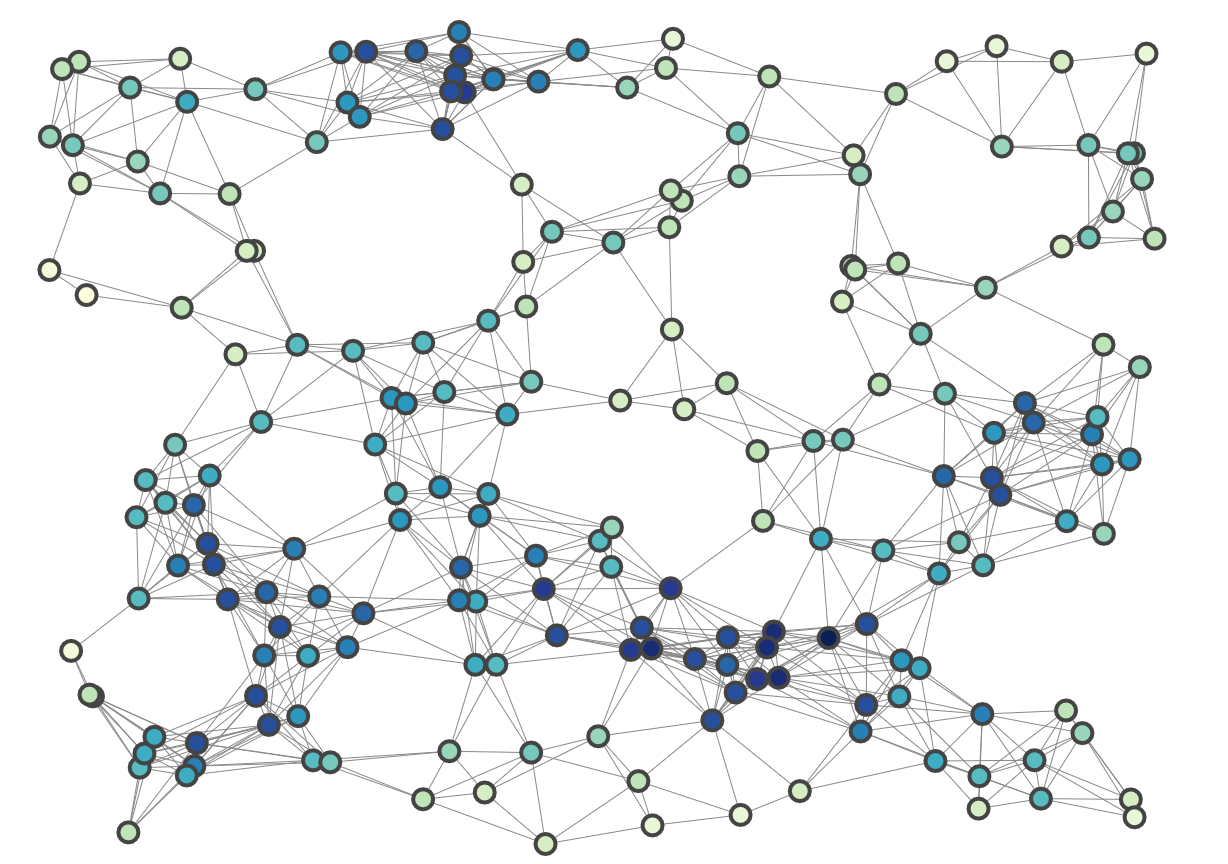
\includegraphics[width=0.5\textwidth]{network_graph}
\end{figure}
Then using a clustering algorithm, find major clusters. These clusters represent ideas. The hashtags that are most in the centre of these clusters describe the purest form of the idea. Label each cluster by this.\\
\\ 
\\ From the clusters of ideas found, ideas or trends that reach their peak popularity among twitter users in a relatively short amount of time and slump in popularity soon after will be the focus of the first part of the project. The reason is that ideas or trends of this kind might resemble a disease outbreak making it possible to use SIR like model to model spread dynamic in time. Moreover, it might be possible to extract contagiousness or contact rate for a given idea or trend. Further analysis can be done to compare contagiousness in different geographical areas and across political spectrum or to break down the features make up this type of ideas.
\\\\
Next we must try to describe the underlying diffusion between these ideas. The SIR model for describing the spread of disease is ideal for this situation. The only two major adjustment that have to be made is that often ideas compete, and also that adopting an idea is a gradual process. You may not start spreading a newly acquired idea immediately as vocally as a long-time supporter. 






% There would for example be the idea of pro-abortion and anti-abortion. Therefore we would have an SIResque model that has the S, which are the susceptible, I which are the infected, and D which are the disbelievers. One problem that has to be resolved, is how to find opposing ideas.
%\[
%  \begin{cases}
%                                   \dot{S} &= \Lambda - \beta S \frac{1}{N} - bS \frac{Z}{N} - \mu S, \\
%                                   \dot{I} &= \beta S \frac{I}{N} - \mu I \\
%                                   \dot{Z} &= bS\frac{Z}{N} - \mu Z
%  \end{cases}
%\]
%where $b$ and $\beta$ denote the per capita rates of idea rejection and adoption by susceptible respectively. $\Lambda$ is the recruitment rate, 

\end{document}